\documentclass[border=6pt]{standalone}
\usepackage{tikz}
\usepackage[edges]{forest}
\usetikzlibrary{arrows.meta,positioning,calc,decorations.pathreplacing,shapes.geometric}
\begin{document}
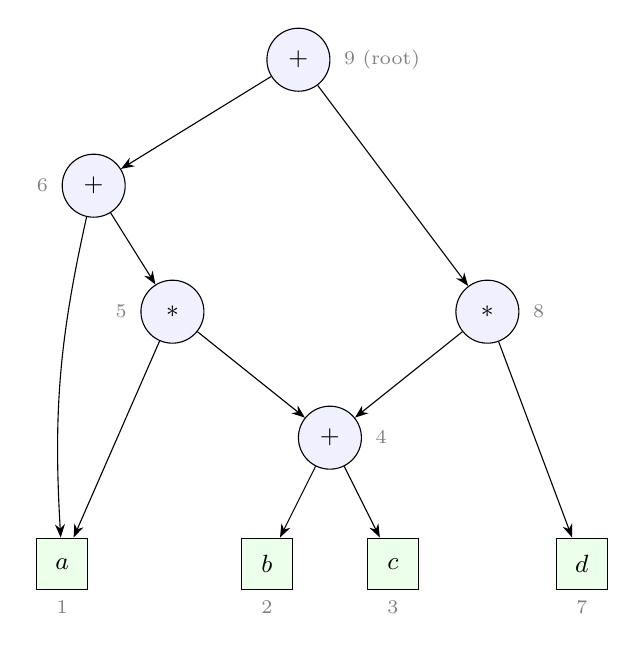
\begin{tikzpicture}[>=Stealth,font=\small,
 op/.style={draw,circle,minimum size=0.8cm,inner sep=0pt,fill=blue!6},
 lf/.style={draw,rectangle,minimum size=0.65cm,inner sep=0pt,fill=green!8},
 nn/.style={font=\scriptsize,gray}]
\node[lf] (a) at (0,0) {$a$}; \node[nn,below=0.02cm of a] {1};
\node[lf] (b) at (2.6,0) {$b$}; \node[nn,below=0.02cm of b] {2};
\node[lf] (c) at (4.2,0) {$c$}; \node[nn,below=0.02cm of c] {3};
\node[lf] (d) at (6.6,0) {$d$}; \node[nn,below=0.02cm of d] {7};
\node[op] (n4) at (3.4,1.6) {$+$}; \node[nn,right=0.05cm of n4] {4};
\node[op] (n5) at (1.4,3.2) {$*$}; \node[nn,left=0.05cm of n5] {5};
\node[op] (n8) at (5.4,3.2) {$*$}; \node[nn,right=0.05cm of n8] {8};
\node[op] (n6) at (0.4,4.8) {$+$}; \node[nn,left=0.05cm of n6] {6};
\node[op] (n9) at (3.0,6.4) {$+$}; \node[nn,right=0.05cm of n9] {9 (root)};
\draw[->] (n4)--(b); \draw[->] (n4)--(c);
\draw[->] (n5)--(a); \draw[->] (n5)--(n4);
\draw[->] (n8)--(n4); \draw[->] (n8)--(d);
\draw[->] (n6) to[bend right=8] (a); \draw[->] (n6)--(n5);
\draw[->] (n9)--(n6); \draw[->] (n9)--(n8);
\end{tikzpicture}
\end{document}
